\section{Ejercicio 2}

%SI QUIEREN AGREGAR IMAGENES COPIEN EL SIGUIENTE CODIGO
%\begin {center}
%\includegraphics[width=12cm]{./graphEj1.jpg}
% grafico.eps: 0x0 pixel, 300dpi, 0.00x0.00 cm, bb=50 50 410 302
%\end {center}
\begin {center}
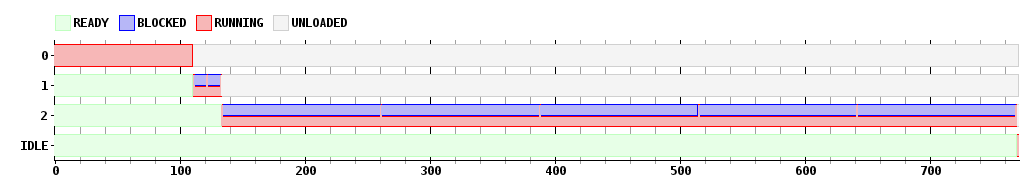
\includegraphics[width=16cm]{../simusched/outputs/outEj2.png}
\end {center}


En el diagrama se puede observar como el scheduler ejecuta las tareas en el orden em que entraron. Esto es debido al tipo de scheduler que utilizamos para correr el lote de tareas, este scheduler (FIFO / FCFS) además de ejecutar las tareas en el orden de entrada, no cambia de tarea hasta que la que esta ejecutando termine. 

Por esto se puede observar que la primera tarea realiza 110 ciclos de reloj y recién después pasa a la próxima tarea. Esto es porque la primera tarea que se ejecuta es "TaskCPU 110" la cual realiza exactamente 110 ciclos de reloj. Lo mismo sucede con las otras 2 tareas, se ejecutan por comleto y no hace el switch hasta finalizar la tarea acutal.

Finalmente vale destacar que las tareas interactivas cumplen lo pedido ya que la primera tarea ejecuta 2 bloqueos de aproximadenete 25 ciclos y la segunda 5 bloqueos de aproximadamente 110 ciclos cada uno. Lo que se ajusta los parametros de entrada ya que la primera tarea tiene un rango de duracion por ciclo de entre 1 y 50 y la segunda entre 100 y 150.
